% sections/05_next_steps.tex: generated by newdeck/html2beamer.py from the HTML deck, then edited by hand
% ---------------------------------------------------------------- slide 34: Outline
\begin{btframe}{}{Outline}
\begin{outlinelist}
\outlineitem{1}{Introduction}{the background types, the geometry, the input muons and neutrinos}{0.35}
\outlineitem{2}{Simulation}{transport, inelastic scattering, technologies, hits and digitisation, signal generation}{0.35}
\outlineitem{3}{Selection}{track cuts, pair cuts and time coincidence}{0.35}
\outlineitem{4}{Backgrounds before tagging}{μ and ν inelastic scattering, MS7 K\textsubscript{L}, combinatorial pairs}{0.35}
\outlineitem{5}{Background tagging}{rules, V0 rule, SBT model, R1, R2, summary}{0.35}
\outlineitem{6}{Optimisation and conclusion}{genetic-algorithm search, the optimised design Z1}{1.00}
\end{outlinelist}
\end{btframe}




% ---------------------------------------------------------------- slide 35: design optimisation with a genetic algorithm (19 Nov 2026)
\begin{btframe}{6 · Optimisation · method}{Design optimisation: a genetic algorithm on the full chain}
\begin{minipage}[t]{0.56\linewidth}\vspace{0pt}
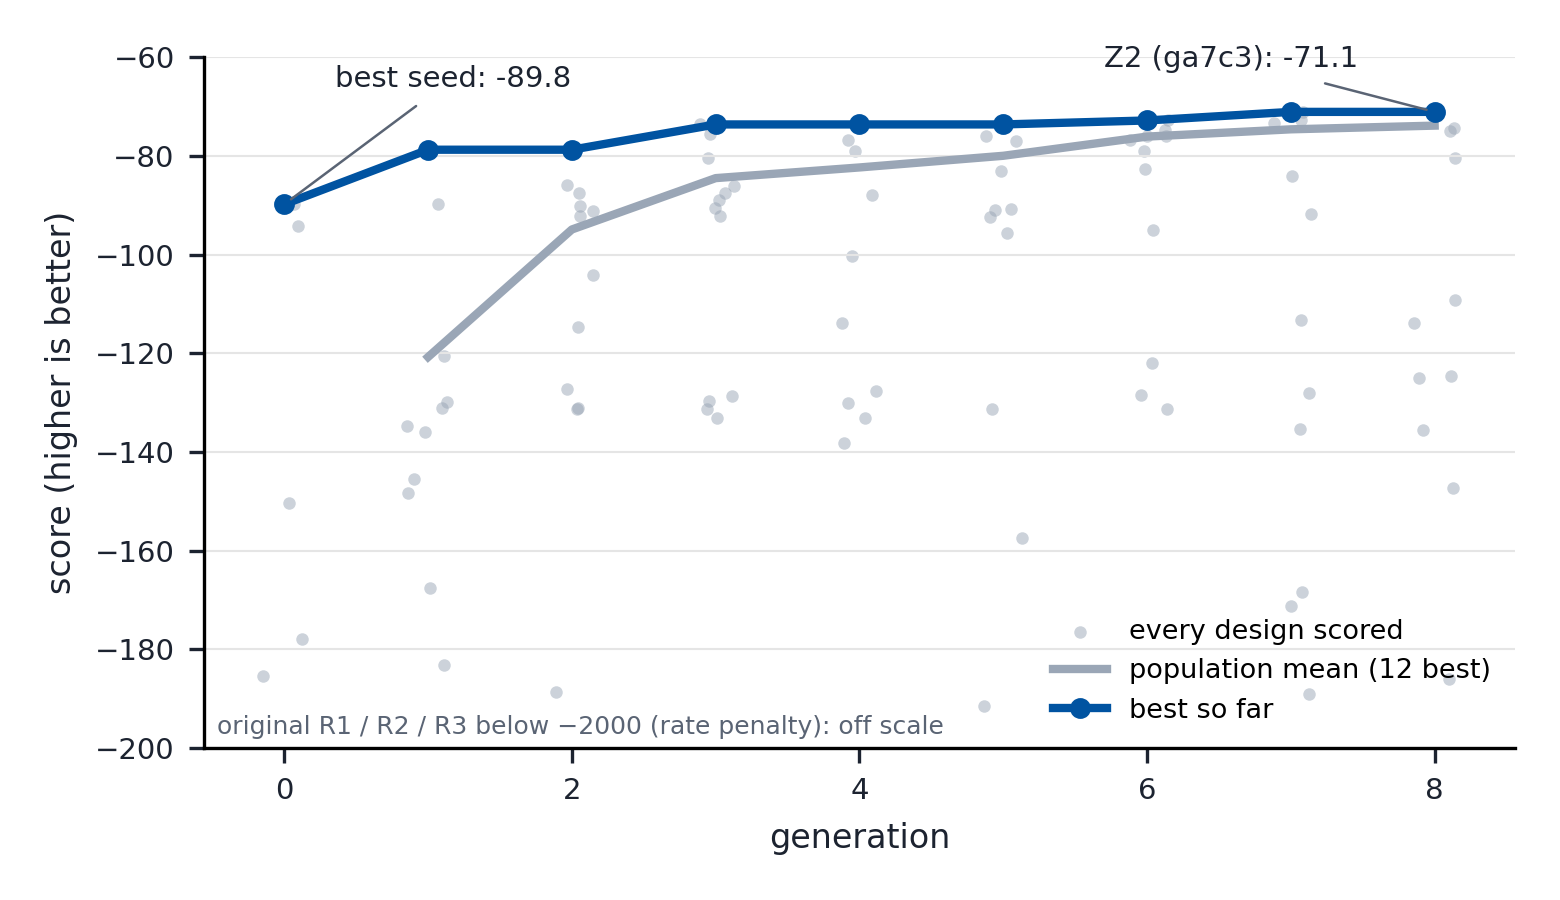
\includegraphics[width=\linewidth]{figs/s35_ga_convergence.png}
\end{minipage}\hfill
\begin{minipage}[t]{0.41\linewidth}\vspace{2pt}

\begin{figure}
    \centering
    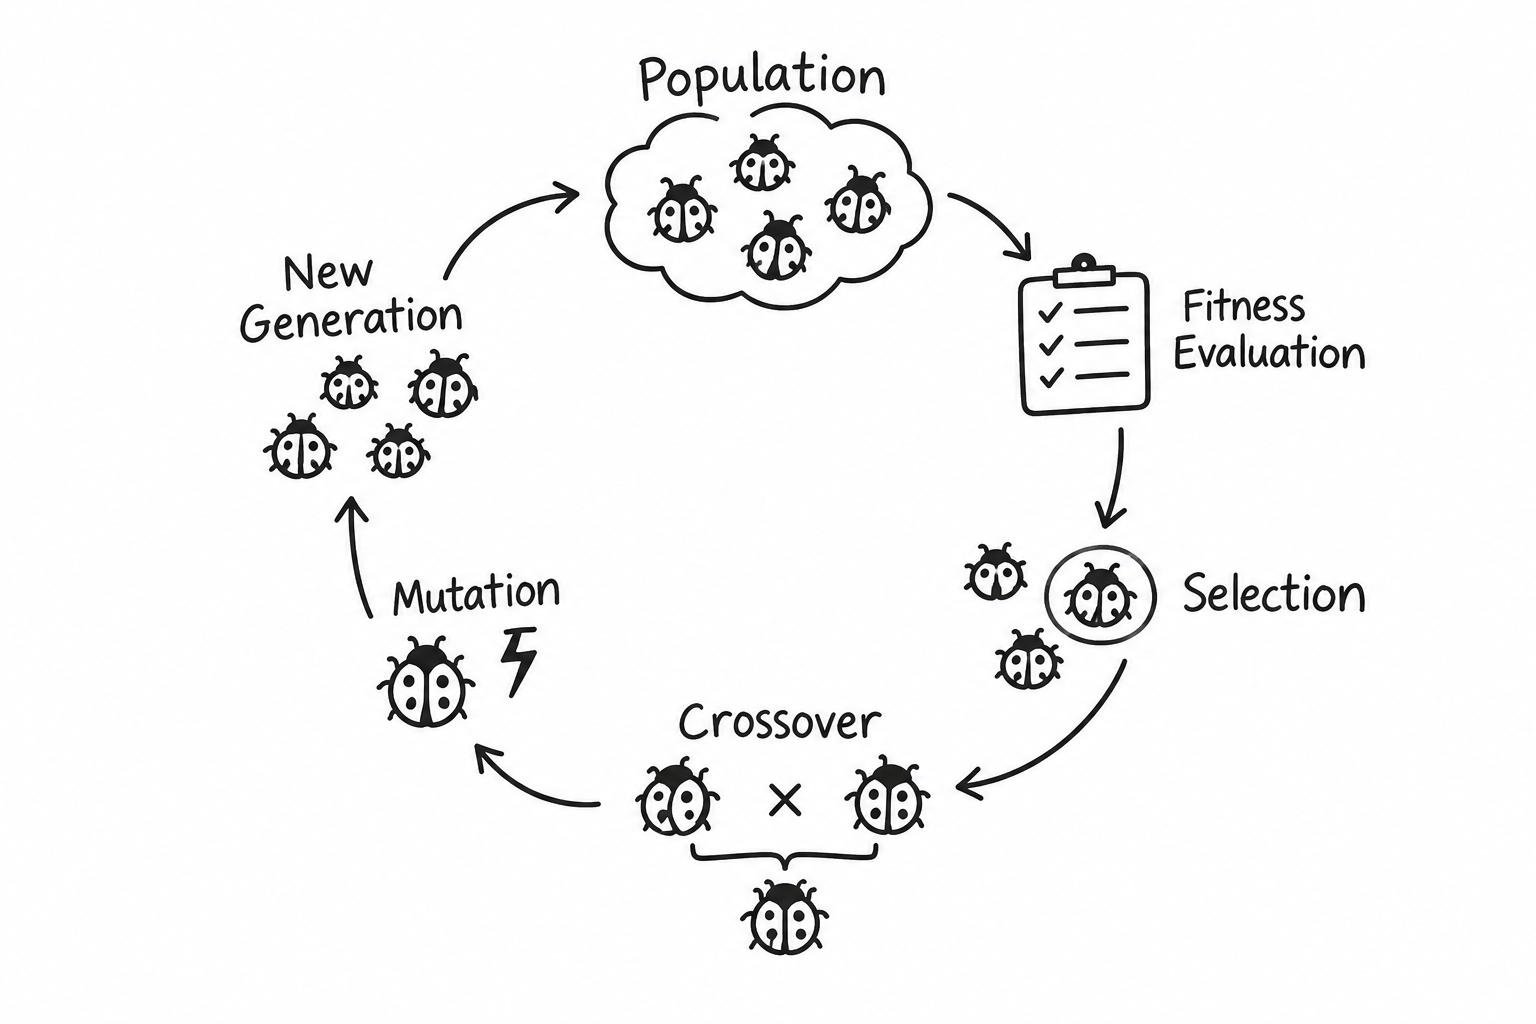
\includegraphics[width=1\linewidth]{figs/GA.png}
\end{figure}
\end{minipage}

{\fontsize{6.15pt}{8.60pt}\selectfont
\begin{itemize}
  \item \textbf{Genes}: SBT rings and threshold, UBT straw extent, tile plane size and 2×2 / 4×4 cm regions, V0 rule settings
  \item \textbf{Each generation}: 12 children by crossover + mutation, scored on Slurm with the chain of this talk (10\textsuperscript{5} signal decays); keep the 12 best
  \item \textbf{Score}: background left, signal lost, cost, rate limits; and the untagged fraction of bounced single SST1 muons
  \item \textbf{Seeds}: the reference designs and R1 / R2 with a 3.4 m tile plane, 2×2 cm only in the cavern-side flame block
  \item Model fixed; V0 p\textsubscript{max} cut held on
\end{itemize}}

\end{btframe}




% ---------------------------------------------------------------- slide 31: Z1: R2 without the SBT, 7 straw fins per side — 439.7 drachmas, 193 368 channels
\begin{btframe}{6 · Optimisation · Z1}{Z1 (optimised): SBT 6 rings + UBT + V0 rule — 225.3 drachmas, 21 171 channels}
{\centering {\renewcommand{\skubtlabel}{UBT: straws + tiles |x| < 1.7 m, 2 × 2 cm\textsuperscript{2} only on the cavern side}\designsketch[74.52pt]{2,5,6,7,8,9}{0}{SBT: rings 2, 5–9 (6 of 10)}}\par}
\vspace{2.46pt}
\noindent \begin{minipage}[c]{0.5\linewidth}
{\fontsize{5.31pt}{6.90pt}\selectfont\setlength{\tabcolsep}{3.72pt}\renewcommand{\arraystretch}{1.42}
\begin{tabular}{lr}
\textcolor{muted}{per 15 y, full selection} & \textcolor{muted}{Z1} \\\headrule
signal lost, full / partial IP cut & 2.79 / 2.43 \% \\\rowrule
μμ pairs & < 0.11 (90 \% CL) \\\rowrule
rock × μ pairs & (1.2 ± 0.9)×10\textsuperscript{-5} \\\rowrule
interaction product × μ pairs & 0.0012 ± 0.0002 \\\rowrule
μ in the vessel & 1.3 ± 1.3 (1 ev.) \\\rowrule
ν in the vessel & 0.94 ± 0.09 \\\rowrule
SBT material μ & 0.001 ± 0.001 \\\rowrule
\rowcolor{tint}\bfseries MS7 μ (V0, K\textsuperscript{±}) & \bfseries 157 ± 58 (27 ev.) \\\rowrule
ν in MS7 / SBT material ν & 0.86 / < 7×10\textsuperscript{-3} \\\rowrule
\rowcolor{tint}\bfseries total background left & \bfseries 160 ± 58 \\\rowrule
single SST1 μ tagged, all / bounced & 92 / 82 \% \\\rowrule
\end{tabular}\par}
\end{minipage}%
\hfill%
\begin{minipage}[c]{0.5\linewidth}
{\fontsize{6.15pt}{8.60pt}\selectfont
\begin{itemize}
  \item Best design of the genetic-algorithm search (section 6): R2 with 6 of the 10 SBT rings (no 0, 1, 3, 4)
  \item UBT straws with t\textsubscript{0} and the segment cut; tile plane |x| < 1.7 m, 2×2 cm only on the cavern side
  \item V0 rule: 0.24 GeV / p\textsubscript{vis} (kinematic limit + 5 \%; the search's 15.7 mrad floor removed), no K\textsubscript{L} time-of-flight window, only for p\textsubscript{vis} < 25 GeV
  \item \textbf{Signal loss 2.8 \%} (R2: 6.1 \%), 68 \% of the budget; every plane within its rate limit
  \item \textbf{With ×4 MS7 statistics: 160 MS7 K\textsubscript{L} left} (R2: 0.74): found on the ×1 sample, it exploited a low-statistics hole → GA re-run
\end{itemize}}
\end{minipage}\par
\end{btframe}


% % ---------------------------------------------------------------- slide 35b: optimisation result
% \begin{btframe}{6 · Optimisation · result}{Optimised designs Z2 and Z3: same tagging, half the signal loss, 68–73 \% of the budget}
% {\fontsize{5.31pt}{6.90pt}\selectfont\setlength{\tabcolsep}{3.72pt}\renewcommand{\arraystretch}{1.42}
% \begin{tabularx}{\linewidth}{>{\raggedright\arraybackslash}Xrrr}
% \textcolor{muted}{per 15 y, full selection} & \textcolor{muted}{R2, 3.4 m tiles (seed)} & \textcolor{muted}{\textbf{Z2} (ga7c3)} & \textcolor{muted}{Z3 (ga8c8)} \\\headrule
% cost, drachmas (\% of budget) & 303.8 (91 \%) & \textbf{225.3 (68 \%)} & 244.7 (73 \%) \\\rowrule
% SBT rings & all 10 & 2, 5–9 & 2, 3, 5–9 \\\rowrule
% V0 cone / time-of-flight window & 25 mrad / on & 15.7 mrad / off & 15.7 mrad / off \\\rowrule
% μ in the vessel & 1.3 (1 ev.) & 1.3 (1 ev.) & 1.3 (1 ev.) \\\rowrule
% SBT material & 2.95 ± 2.99 (1 heavy ev.) & 0.004 & 0.004 \\\rowrule
% MS7 μ (V0, K\textsuperscript{±}) & 0.59 ± 0.25 & 0.80 ± 0.34 & 0.61 ± 0.27 \\\rowrule
% ν in the helium & 1.08 & 1.13 & 1.05 \\\rowrule
% single SST1 tagged, all / bounced & 94 / 83 \% & 91 / 84 \% & 94 / 84 \% \\\rowrule
% \rowcolor{tint}\bfseries signal lost & \bfseries 5.94 \% & \bfseries 2.71 \% & \bfseries 3.01 \% \\\rowrule
% \end{tabularx}\par}
% \vspace{2.46pt}
% {\fontsize{6.15pt}{8.60pt}\selectfont
% \begin{itemize}
%   \item Solid: signal loss halved (5.9 → 2.7 \%) and −79 drachmas, with the bounced-muon tagging kept; every plane within its rate limit
%   \item The SBT-material gain is one heavy simulated event: not a measured improvement
%   \item All three keep the same changes: rings 0, 1, 4 off, straw t\textsubscript{0} + segment cut, tighter V0 cone
% \end{itemize}}
% \end{btframe}

% ---------------------------------------------------------------- slide 36: Conclusion
\begin{btframe}{6 · Next steps · conclusion}{Conclusion}
\noindent\begin{minipage}[t]{0.49\linewidth}\vspace{0pt}
\begin{mathbox}[cern]{7pt}
{\fontsize{8.6pt}{10pt}\selectfont\textbf{\textcolor{cern}{1 · Simulation environment: fast and efficient}}}\par\vspace{2pt}
\begin{itemize}\setlength{\itemsep}{3pt}
  \item Cuda Muons: 3.2×10\textsuperscript{6} μ/s on one GPU, ≈ 4×10\textsuperscript{5} × FairShip per core: \textbf{3 220 spills} of muons simulated
  \item Forced inelastic interactions: every crossing gives an event; 2×10\textsuperscript{7} MS7 interactions in 14 min
  \item Full chain per design (all backgrounds + 10\textsuperscript{5} signal decays) in \textbf{72 s} on one core
\end{itemize}
\end{mathbox}
\end{minipage}\hfill\begin{minipage}[t]{0.49\linewidth}\vspace{0pt}
\begin{mathbox}[purple]{7pt}
{\fontsize{8.6pt}{10pt}\selectfont\textbf{\textcolor{purple}{2 · Selection and tagging strategy (preliminary)}}}\par\vspace{2pt}
\begin{itemize}\setlength{\itemsep}{3pt}
  \item Good track: p > 1 GeV, all 4 straw stations + TD; pair: opposite charge, DOCA < 1 cm, vertex in the vessel, IP < 10 cm (full) / 2.5 m (partial)
  \item Tagging, all rules at once (OR): track back-trace window, V0 rule (kinematic disc 0.24 GeV / p\textsubscript{vis}, p\textsubscript{vis} < 25 GeV), SBT rules
  \item Background tagged with its own hits only; random hits only for the signal loss
\end{itemize}
\end{mathbox}
\end{minipage}
\vspace{10pt}
\noindent\begin{minipage}[t]{0.49\linewidth}\vspace{0pt}
\begin{mathbox}[green]{7pt}
{\fontsize{8.6pt}{10pt}\selectfont\textbf{\textcolor{green}{3 · FairShip designs evaluated in the framework}}}\par\vspace{2pt}
\begin{itemize}\setlength{\itemsep}{3pt}
  \item \textbf{R1} (UBT only, 99.7 drachmas): (1.33 ± 0.08)×10\textsuperscript{4} / 15 y left, MS7 K\textsubscript{L} dominated; signal lost 2.3 \%
  \item \textbf{R2} (SBT + UBT + V0 rule, the budget): 4.3 ± 1.4 / 15 y left; signal lost 6.1 / 9.0 \% (full / partial)
  % \item MS7 K\textsubscript{L} with 4× statistics: R2 term 0.74 ± 0.23 with the V0 rule at the kinematic limit + 5 \%
\end{itemize}
\end{mathbox}
\end{minipage}\hfill\begin{minipage}[t]{0.49\linewidth}\vspace{0pt}
\begin{mathbox}[orange]{7pt}
{\fontsize{8.6pt}{10pt}\selectfont\textbf{\textcolor{orange}{4 · Next steps}}}\par\vspace{2pt}
\begin{itemize}\setlength{\itemsep}{3pt}
  \item Optimisation with \textbf{AlphaEvolve} on the full chain: a first evaluation of the figure of merit has been done (genetic-algorithm trial Z1: 2.8 \% signal loss at 68 \% of the budget)
  %but 160 MS7 K\textsubscript{L} with 4× statistics: re-run on the ×4 sample)
  \item Enriched samples for the one-event classes (vessel μ, MS7 K\textsubscript{L}); track-window study (simulation-based r(p))
  \item FairShip validation of the optimum
\end{itemize}
\end{mathbox}
\end{minipage}
\end{btframe}
